\documentclass[10pt,a4paper, titlepage]{report}

% Pacchetti...
% ----------------------------------------------------------------------------------------- %
\usepackage[utf8]{inputenc}
\usepackage[italian]{babel}
\usepackage{booktabs}
\usepackage{amsmath}
\usepackage{amsfonts}
\usepackage{amssymb}
\usepackage{listings}
\usepackage{xcolor}
\usepackage{graphicx}
\usepackage{sidecap}
\usepackage{float}
\usepackage{siunitx}
\usepackage{multirow}
\usepackage{hyperref}
\usepackage{bmpsize}
\usepackage{adjustbox}
\usepackage{footnote}
\usepackage{authblk}
\usepackage{titlesec}
\usepackage{frontespizio} 


\titleformat{\paragraph}
{\normalfont\normalsize\bfseries}{\theparagraph}{1em}{}
\titlespacing*{\paragraph}
{0pt}{3.25ex plus 1ex minus .2ex}{1.5ex plus .2ex}



\usepackage{tabularx}
\usepackage[skip=0.5\baselineskip]{caption}


% Usato per personalizzare l'ambiente 'listings'...
% ----------------------------------------------------------------------------------------- %
\lstset{
language=C,
basicstyle=\small\ttfamily,			
keywordstyle=\color{blue},
commentstyle=\color{gray},			
stringstyle=\color{black},			
numbers=left,						
numberstyle=\tiny,					
stepnumber=1,						
breaklines=true						
}

% Usato per aggiugnere la numerazione alle sezioni di tipo 'subsubsection' e inserirle nell'indice...%
\setcounter{secnumdepth}{4}
\setcounter{tocdepth}{4}

\usepackage{lipsum}
\usepackage{suffix}

\newcommand\chapterauthor[1]{\authortoc{#1}\printchapterauthor{#1}}
\WithSuffix\newcommand\chapterauthor*[1]{\printchapterauthor{#1}}

\newcommand\sectionauthor[1]{\authorsectiontoc{#1}\printsectionauthor{#1}}
\WithSuffix\newcommand\sectionauthor*[1]{\printsectionauthor{#1}}

\newcommand\sectionsecondauthor[1]{\authorssecondectiontoc{#1}\printsectionsecondauthor{#1}}
\WithSuffix\newcommand\sectionsecondauthor*[1]{\printsectionsecondauthor{#1}}

\makeatletter
\newcommand{\printchapterauthor}[1]{%
  {\parindent0pt\vspace*{-25pt}%
  \linespread{1.1}\large\scshape#1%
  \par\nobreak\vspace*{35pt}}
  \@afterheading%
}
\newcommand{\printsectionauthor}[1]{%
  {\parindent0pt\vspace*{-10pt}%
  \linespread{1.1}\large\scshape#1%
  \par\nobreak\vspace*{20pt}}
  \@afterheading%
}
\newcommand{\printsectionsecondauthor}[1]{%
  {\parindent0pt\vspace*{-20pt}%
  \linespread{1.1}\large\scshape#1%
  \par\nobreak\vspace*{20pt}}
  \@afterheading%
}
\newcommand{\authortoc}[1]{%
  \addtocontents{toc}{\vskip-10pt}%
  \addtocontents{toc}{%
    \protect\contentsline{chapter}%
    {\hskip1.3em\mdseries\scshape\protect\scriptsize#1}{}{}}
  \addtocontents{toc}{\vskip5pt}%
}
\newcommand{\authorsectiontoc}[1]{%
  \addtocontents{toc}{\vskip-10pt}%
  \addtocontents{toc}{%
    \protect\contentsline{chapter}%
    {\hskip1.3em\mdseries\scshape\protect\scriptsize#1}{}{}}
  \addtocontents{toc}{\vskip5pt}%
}
\newcommand{\authorssecondectiontoc}[1]{%
  \addtocontents{toc}{\vskip-14pt}%
  \addtocontents{toc}{%
    \protect\contentsline{chapter}%
    {\hskip1.3em\mdseries\scshape\protect\scriptsize#1}{}{}}
  \addtocontents{toc}{\vskip5pt}%
}
\makeatother

\date{27 marzo 2019}

% Inzio documento...
% ----------------------------------------------------------------------------------------- %
\begin{document}

% Frontespizio
% ------------------------------------------------------
\begin{frontespizio} 
\Universita{Roma ``Tor Vergata'' } 
\Logo[3cm]{logo}
\Facolta{Ingegneria} 
\Corso[Laurea Magistrale]{Ingegneria Informatica} 
\Annoaccademico{2018--2019} 
\Titolo{Il malware FASTCash \\ \small{Sicurezza informatica e Internet}}
\NCandidato{Studente} 
\Candidato[0273395]{Andrea Graziani} 
\Candidato[0277414]{Alessandro Boccini} 
\Candidato[0274716]{Ricardo Gamucci} 

\NRelatore{Docente}{} 
\Relatore{Maurizio Naldi} 
\end{frontespizio} 

\tableofcontents
\newpage

\chapter{Introduzione}
\chapterauthor{\small{\textit{Autore:} \textbf{Andrea Graziani} (\textbf{0273395})}}

Lo scopo della presente relazione è quella di fornire un'analisi il più possibile dettagliata del malware denominato \textbf{FASTCash}\footnote{\texttt{https://www.symantec.com/security-center/writeup/2018-110615-2942-99}} la cui paternità, secondo le analisi forensi eseguite da varie aziende ed agenzie, tra cui la \textbf{Symantec}, \textbf{Kaspersky} e la \textbf{NCCIC}\footnote{Stiamo parlando della "\textit{National Cybersecurity and Communications Integration Center}" un'agenzia federale americana specializzata in sicurezza informatica facente parte della CISA (\textit{Cybersecurity and Infrastructure Security Agency}) \\ Per ulteriori informazioni in merito si veda: \texttt{https://www.us-cert.gov/about-us} }, è attribuita ad un gruppo di cyber-criminali conosciuto come \textit{Lazarus Group}\footnote{\texttt{https://www.symantec.com/blogs/threat-intelligence/fastcash-lazarus-atm-malware}} \footnote{\texttt{https://www.us-cert.gov/ncas/alerts/TA18-275A}}, di cui forniremo una descrizione più dettagliata nella sezione \ref{lazarausgrpo}.

La scoperta del malware risale precisamente al \textbf{2 ottobre 2018} giorno in cui, grazie al lavoro congiunto effettuato da varie agenzie ed istituzioni americane, tra cui \textbf{FBI}, \textbf{Dipartimento del Tesoro Americano} e la \textbf{DHS} (\textit{Department of Homeland Security})\footnote{\textit{Ibidem}}, venne pubblicato sul sito del CISA l'avviso \texttt{TA18-275A}, secondo la quale esponenti del gruppo Lazarus avevano condotto con successo una serie di attacchi, denominati dalla CISA come \textit{FASTCash}, per il\textbf{ prelievo fraudolento di denaro contante dagli ATM} (\textit{Automated Teller Machines}) di varie banche in oltre 30 paesi diversi sparsi fra Asia e Africa \footnote{\textit{Ibidem}}. E' importante sottolineare che, sebbene l'esistenza del malware sia stata resa di dominio pubblico solo allora, la CISA ha dichiarato che il gruppo Lazarus ha condotto attacchi di tipo FASTCash già a partire dal 2016.

Per essere precisi, come si evince dal rapporto \texttt{AR18-275A} pubblicato dalla CISA\footnote{Cfr. \texttt{https://www.us-cert.gov/ncas/analysis-reports/AR18-275A}}, il malware FASTCash è in realtà composto da un'insieme di \textbf{12 file}, ognuno dei quali avente un ruolo e uno scopo specifico. Abbiamo riportato per comodità una lista completa dei file di FASTCash in \ref{tab:MalwareFileList}; tre di essi sono stati analizzati in dettaglio nel capitolo \ref{processoinjection}.

\begin{table}[h!]
 
    \caption{Lista dei file del malware FASTCash}
    \centering
    \small
    \label{tab:MalwareFileList}
    
    \begin{adjustbox}{center=\textwidth}
 
     \begin{tabular}{l|r}
      \toprule
      \textbf{Nome file} & \textbf{SHA256 digest} \\
      \midrule
      
      Lost\_File.so & \texttt{10ac312c8dd02e417dd24d53c99525c29d74dcbc84730351ad7a4e0a4b1a0eba} \\
      \hline
      Unpacked\_dump\_4a740227eeb82c20... & \texttt{10ac312c8dd02e417dd24d53c99525c29d74dcbc84730351ad7a4e0a4b1a0eba} \\
  \hline
  Lost\_File1\_so\_file & \texttt{3a5ba44f140821849de2d82d5a137c3bb5a736130dddb86b296d94e6b421594c} \\
    \hline
      4f67f3e4a7509af1b2b1c6180a03b3... & \texttt{4a740227eeb82c20286d9c112ef95f0c1380d0e90ffb39fc75c8456db4f60756} \\ 
      \hline
      5cfa1c2cb430bec721063e3e2d144f... & \texttt{820ca1903a30516263d630c7c08f2b95f7b65dffceb21129c51c9e21cf9551c6} \\
      \hline
      Unpacked\_dump\_820ca1903a305162... & \texttt{9ddacbcd0700dc4b9babcd09ac1cebe23a0035099cb612e6c85ff4dffd087a26} \\
      \hline
      8efaabb7b1700686efedadb7949eba... & \texttt{a9bc09a17d55fc790568ac864e3885434a43c33834551e027adb1896a463aafc} \\
      \hline
      d0a8e0b685c2ea775a74389973fc92... & \texttt{ab88f12f0a30b4601dc26dbae57646efb77d5c6382fb25522c529437e5428629} \\
      \hline
      2.so & \texttt{ca9ab48d293cc84092e8db8f0ca99cb155b30c61d32a1da7cd3687de454fe86c} \\
      \hline
      Injection\_API\_executable\_e & \texttt{d465637518024262c063f4a82d799a4e40ff3381014972f24ea18bc23c3b27ee}\\
      \hline
      Injection\_API\_log\_generating\_s & \texttt{e03dc5f1447f243cf1f305c58d95000ef4e7dbcc5c4e91154daa5acd83fea9a8}\\
      \hline
      inject\_api & \texttt{f3e521996c85c0cdb2bfb3a0fd91eb03e25ba6feef2ba3a1da844f1b17278dd2}\\
      
      \bottomrule
    \end{tabular}
    \end{adjustbox}
  
\end{table}

\section{Descrizione generale dell'attacco}\label{descr}

Per effettuare con successo un attacco FASTCash, i cyber-criminali violavano dapprima le reti delle banche bersaglio allo scopo di ottenere accesso completo ai cosiddetti \textbf{server di payment switch} (\textit{switch application servers}), i server responsabili della gestione delle transazioni finanziare tra gli ATM e il sistema informatico principale della banca.\footnote{\texttt{https://www.symantec.com/blogs/threat-intelligence/fastcash-lazarus-atm-malware}}

Si presuppone che gli attaccanti, al fine di ottenere accesso alle suddette reti, abbiano adottato tecniche di \textbf{spear-phishing}\footnote{\texttt{https://securityaffairs.co/wordpress/76798/hacking/fastcash-hidden-cobra-attacks.html}}, ossia una serie di attacchi di \textit{phishing} che, a differenza di quelli più comuni, hanno come bersaglio individui \textit{specifici}, vale a dire persone di cui gli attaccanti potevano conoscere diverse informazioni (nome, sesso, ruolo, abitudini, ecc.) al fine di aumentare le probabilità di successo \footnote{\texttt{https://www.kaspersky.it/resource-center/definitions/spear-phishing}}. 

\begin{figure}[h!]
    \centering
    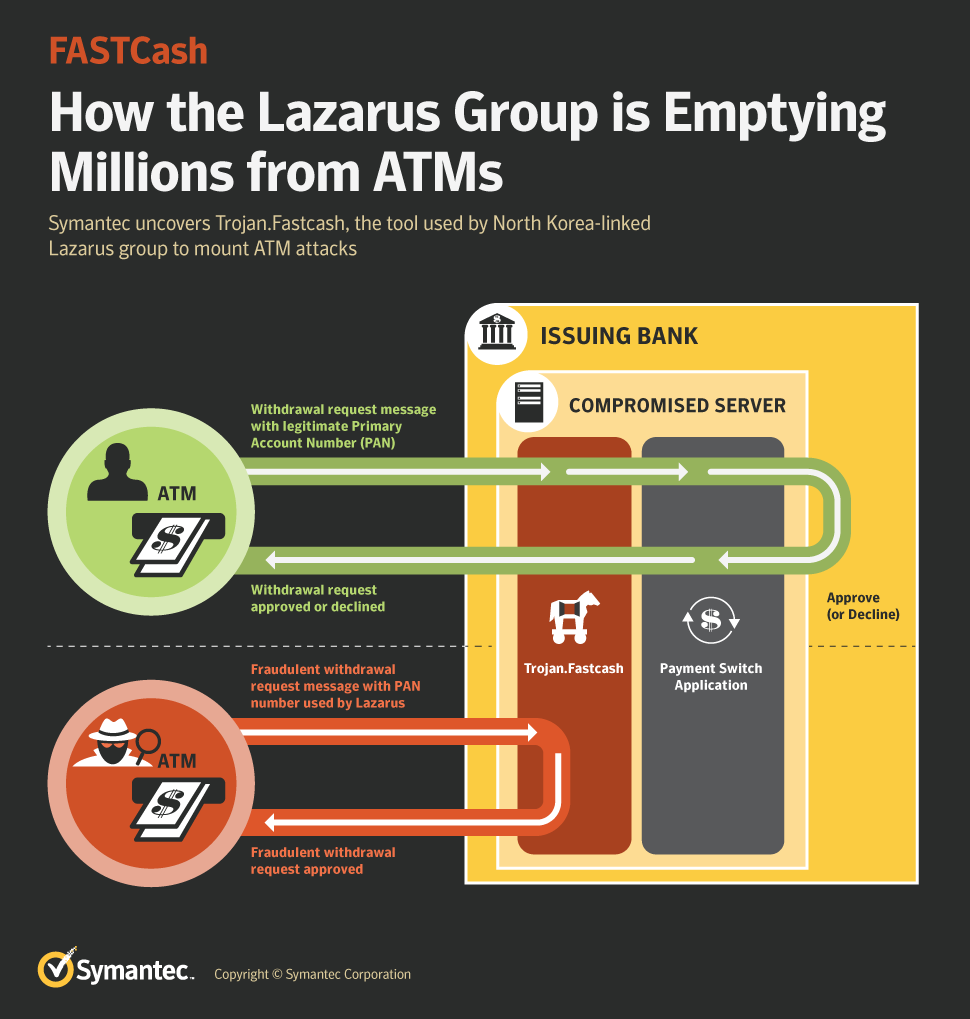
\includegraphics[width=\textwidth]{./FASTCash.png} 
\end{figure}

Il vero scopo dei suddetti attacchi di phishing riguardava l'installazione, nel computer della vittima, del malware denominato \texttt{5cfa1c2cb430bec721063e3e2d144feb} (la stringa \textbf{MD5} ad esso associata) il cui scopo, secondo le analisi condotte dalla NCCIC, era colpire i sistemi operativi Windows dei dipendenti della banca in modo tale da consentire agli attaccanti l'accesso in remoto al sistema bancario\footnote{\texttt{https://www.us-cert.gov/ncas/analysis-reports/AR18-275A}}.

Per conseguire tale scopo, il suddetto malware eseguiva una serie di operazioni tra cui:

\begin{itemize}
\item Alterare le impostazioni di \textit{Windows Firewall} allo scopo di consentire l'instaurazione di connessioni TCP verso la macchina dall'esterno.\footnote{\textit{Ibidem}}
\item Caricare in memoria uno speciale \textbf{modulo proxy} che, secondo la NCCIC, oltre ad essere stato progettato ad agire come una \textit{command-line utility}, forzava la macchina ad agire come se fosse un proxy server, consentendo agli attaccanti di interagire in remoto con il malware.\footnote{\textit{Ibidem}}
\end{itemize}

Le analisi condotte dalla NCCIC hanno dimostrato che gli attaccanti, per mezzo del suddetto malware, sono riusciti a trasferire un \textbf{injection tool} all'interno dei sistemi di payment switch al fine di introdurre codice malevolo all'interno di uno o più processi legittimi. 

Il codice introdotto si è rivelato capace di interagire con i messaggi basati sul \textbf{protocollo ISO 8583} scambiati tra gli ATM e il sistema informatico bancario centrale, consentendo agli aggressori di prelevare denaro agli sportelli automatici.

\section{Manipolazioni dei messaggi ISO 8583}
\sectionauthor{\quad\quad\quad \small{\textit{Autore:} \textbf{Alessandro Boccini} (\textbf{0277414})}}
\sectionsecondauthor{\quad\quad\quad \small{\textit{Editing:} \textbf{Andrea Graziani} (\textbf{0273395})}}

L'ISO 8583 è uno standard internazionale di messaggio nell'ambito delle transazioni finanziarie, utilizzato da molte reti finanziarie, tra cui Visa e MasterCard e dalla quasi totalità degli enti finanziari mondiali.

Dal punto di vista strutturale, un messaggio ISO 8583 è composta da 3 campi:

\begin{description}
\item[Message Type Identifier (MTI)] Identifica la tipologia del messaggio ed è composto da un insieme di 4 valori dove:

\begin{itemize}
\item Il primo indica la versione del protocollo il quale, qualora assumesse, ad esempio, il valore 0, denota la versione del 1987 del protocollo.
\item Il secondo è utilizzato per indicare la classe del messaggio; un valore pari a 2 indica un messaggio di tipo finanziario.
\item Il terzo indica, invece, la funzione svolta dal messaggio; un valore pari a 0 è usato per rappresentare una richiesta mentre, se pari ad 1, una risposta.
\item Infine, il quarto è usato per identificare il soggetto della transazione; il valore 0 indica un generico acquirente.
\end{itemize}

\item[Bitmap] Rappresenta un campo composto da 64 bit (o 16 caratteri esadecimali) in cui ogni bit posto a 1 denota la validità delle informazioni presenti nel campo \textit{Data} del messaggio; per esempio, qualora il bit n. 2 assumesse valore pari ad 1, il campo \textbf{PAN} (\textit{Primary Account Number}) risulta essere presente nel payload del messaggio.

\item[Data] Rappresenta il payload contenente tutte le informazioni relative alla transazione. Può contenere fino a 192 possibili elementi (128 nella versione del 1987) ognuno dei quali può contenere dati numerici, alfanumerici o binari di lunghezza fissa o variabile.
\end{description}

\subsection{Manipolazione}

Durante l'attacco, il malware interagisce esclusivamente con i messaggi dove:
\begin{enumerate}
\item Il MTI del messaggio contiene il valore \texttt{0200}, ossia \textit{una richiesta di prelievo di denaro da parte dell'acquirente}.
\item il valore del \textit{Point of service entry modes}, indicante le modalità di accesso al sistema bancario, sia pari a 90, valore che indica l'uso di una carta di credito.
\end{enumerate}

Una volta intercettato un messaggio con tali caratteristiche, il malware estrae il valore corrispondete al campo PAN e lo confronta con un insieme di valori PAN posseduti dagli attaccanti. 

Tale verifica avviene per mezzo di una funzione contenuta all'interno delle librerie introdotte nel sistema; la funzione \texttt{CheckPan()}\footnote{\texttt{https://security.arizona.edu/content/ta18-275a-hidden-cobra-–-fastcash-campaign}} \footnote{\texttt{https://www.symantec.com/blogs/threat-intelligence/fastcash-lazarus-atm-malware}}.

Qualora la verifica abbia avuto esito positivo, ovvero il PAN estratto dal messaggio corrisponde ad uno dei PAN in possesso agli attaccanti, il messaggio viene manipolato invocando la funzione \texttt{GenerateResponseTransaction1}, la quale modifica il terzo valore del campo MIT del messaggio impostandolo ad 1. Infine, il messaggio, con valore MIT pari ad \texttt{0210}, viene inoltrato all'ATM che rilascerà i contanti ai criminali, completando così l'attacco.

In tutti gli altri casi, i messaggi vengono rilasciati e inoltrati al sistema bancario seguendo il normale l'iter.

\section{Gruppo Lazarus}\label{lazarausgrpo}
\sectionauthor{\quad\quad\quad \small{\textit{Autore:} \textbf{Ricardo Gamucci} (\textbf{0274716})}}
\sectionsecondauthor{\quad\quad\quad \small{\textit{Editing:} \textbf{Andrea Graziani} (\textbf{0273395})}}

Il \textit{Lazarus Group}, conosciuto anche come \textit{HIDDEN COBRA} o \textit{Guardians of Peace}, è un gruppo di cyber-criminali, composto da un numero imprecisato di individui, ritenuto responsabile di una serie di attacchi informatici perpetrati a danno di istituti bancari, software house e casino oltre ad una serie di attività legate al mining di cripto-valute.\footnote{\texttt{https://securelist.com/lazarus-under-the-hood/77908/}}

La paternità degli attacchi effettuati dal gruppo è stata dimostrata da Kaspersky Lab, nota azienda attiva nel campo della sicurezza informatica, la quale, attraverso un'analisi forense molto dettagliata sulle attività del gruppo in cui è stato eseguito un confronto minuzioso dei codici assembly estratti dai malware utilizzati in diversi attacchi, ha dimostrato l'uso di uno stesso \textit{core base} attribuito al gruppo stesso.\footnote{\texttt{https://media.kasperskycontenthub.com/wp-content/uploads/sites/43/2018/03/07180244/Lazarus\_Under\_The\_Hood\_PDF\_final.pdf}}

La NCCIC, Kaspersky Lab e la Symantec attribuiscono al gruppo Lazarus la responsabilità di attacchi molto famosi, tra cui spiccano per importanza ed entità il furto di dati a danno della Sony Pictures Entertainment, il furto di denaro dalla Banca Centrale del Bangladesh nonché dei danni provati dal ben noto ransomware WannaCry\footnote{\texttt{https://www.theguardian.com/technology/2017/may/15/wannacry-ransomware-north-korea-lazarus-group}}. 

Per essere precisi, la NCCIC la ritiene colpevole di ben 17 attacchi, tra cui ovviamente FASTCash, sebbene la certezza di tale numero possa essere messa in discussione dal fatto che il governo statunitense attribuisca alla HIDDEN COBRA la quasi totalità degli attacchi provenienti dalla nord-corea.\footnote{\texttt{https://www.us-cert.gov/HIDDEN-COBRA-North-Korean-Malicious-Cyber-Activity}}.

\begin{figure}[h!]
    \centering
    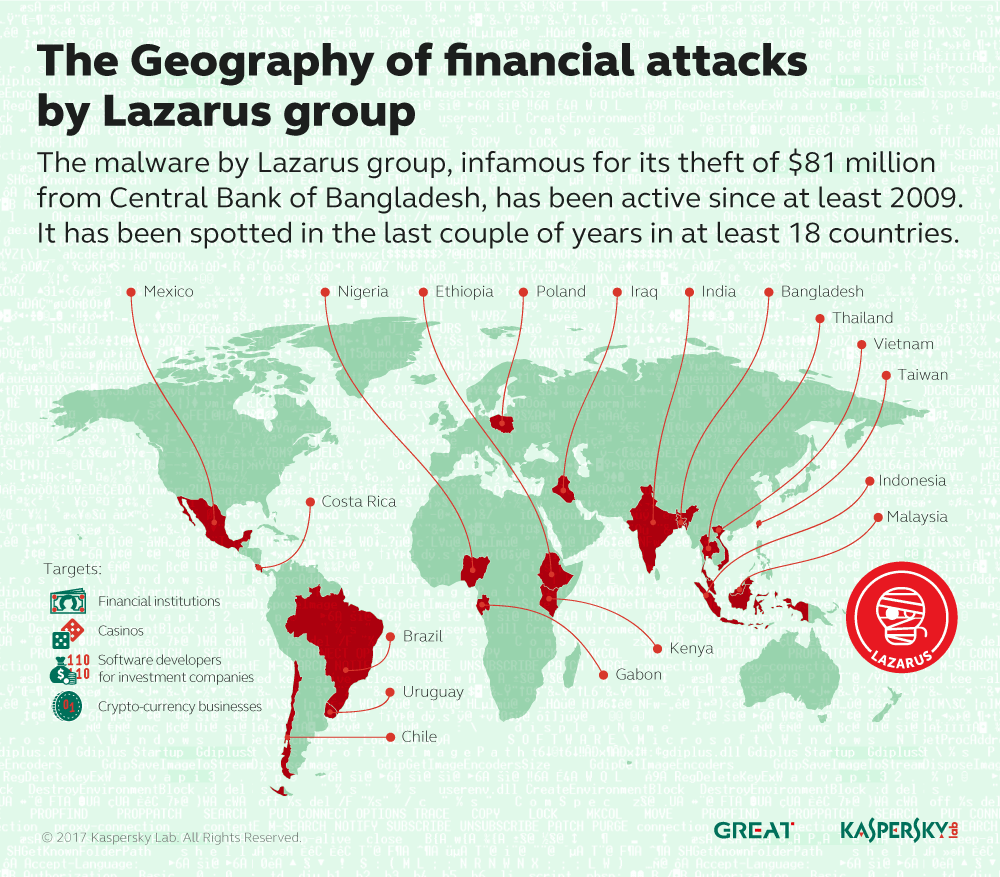
\includegraphics[width=\textwidth]{./img-lazarus-world-attack.png} 
\end{figure}

La presunta origine nordcoreana del gruppo è stata dimostrata, ancora una volta, da Kaspersky; l'azienda, attraverso un'analisi di vari server C2\footnote{\textit{Command-and-control}, indicato a volte con la sigla C\&C o C2, server usati dagli attaccanti per mantenere le comunicazioni con i sistemi compromessi}, localizzati in Europa e usati dal gruppo per le loro attività criminali, ha rilevato l'uso di un piccolo intervallo di indirizzi IP di origine nordcoreana da cui si presuppone avessero origine tutte le richieste di connessione verso i server C2, sebbene queste avvenissero per mezzo di server proxy e connessioni VPN.\footnote{\texttt{https://securelist.com/lazarus-under-the-hood/77908/}}
 
\newpage
\chapter{Analisi dell'attacco di Process Injection}\label{processoinjection}
\chapterauthor{\small{\textit{Autore:} \textbf{Andrea Graziani} (\textbf{0273395})}}

\section{Introduzione}

In questo capitolo analizzeremo dettagliatamente la tecnica di attacco usata dai cyber-criminali per alterare a loro vantaggio il corretto funzionamento dei server bancari presso le quali erano in esecuzione le applicazioni di \textit{payment switch}.

\subsection{Definizione della forma di attacco}

I rapporti pubblicati dalla NCCIC\footnote{\texttt{https://www.us-cert.gov/ncas/analysis-reports/AR18-275A}} \footnote{\texttt{https://www.us-cert.gov/ncas/alerts/TA18-275A}} e dalla Symantec\footnote{\texttt{https://www.symantec.com/blogs/threat-intelligence/fastcash-lazarus-atm-malware}} indicano che la forma di attacco adottata per compromettere i server dell'istituto bancario fosse stata una \textbf{process injection}.

Con la locuzione \textit{process injection} si intende una tecnica che rende possibile \textit{l'esecuzione di codice arbitrario precedentemente introdotto all'interno dello spazio d'indirizzamento di un processo distinto in esecuzione}.\footnote{\texttt{https://attack.mitre.org/techniques/T1055/}}

L'esecuzione di codice maligno nel contesto di un processo legittimo, oltre a garantire ai cyber-criminali l'accesso a tutte le risorse assegnate al suddetto processo da parte del SO (memoria, risorse di rete, dati ecc.), non viene generalmente individuata dai prodotti commerciali per la sicurezza informatica, essendo l'esecuzione del malware \textit{nascosta}.\footnote{\textit{Ibid.}}

\subsection{Descrizione della variante di attacco adottata}

Esistono molte varianti di attacco di process injection che, sfruttando diverse tipologie di vulnerabilità esposte dal sistema operativo, sono in grado di introdurre con successo codice arbitrario all'interno di un processo; la variante adottata dai cyber-criminali nel malware FASTCash è conosciuta come \textbf{SIR}, acronimo di \textbf{Suspend-Inject-Resume}.

Come facilmente intuibile dal nome, tale tipologia di attacco prevede 3 fasi:\footnote{\texttt{https://www.endgame.com/blog/technical-blog/ten-process-injection-techniques-technical-survey-common-and-trending-process}}
\begin{enumerate}
\item La \textbf{sospensione del processo} bersaglio o, più specificatamente, di tutti i suoi thread. 
\item \textbf{Alterazione dello stato del processo} attraverso la modifica del suo spazio di indirizzamento (\textit{Address Space}) o dei valori contenuti nel suo PCB, come il valore che detiene l'indirizzo della successiva istruzione (\textit{Program Counter}/\textit{Instruction Pointer}) o i dati contenuti nei registri.
\item Il \textbf{riavvio del processo} attaccato in modo tale che esegua il codice maligno precedentemente introdotto.
\end{enumerate}

\subsection{Gli strumenti usati per l'analisi}

Prima di procedere con la descrizione dettagliata dell'attacco perpetrato dal malware FASTCash, riportiamo di seguito i vari tool utilizzati durante le nostre analisi:

\begin{description}
\item[\texttt{strings}]\footnote{Cfr. \texttt{https://linux.die.net/man/1/strings}} Usato per l'estrazione di tutte le stringhe stampabili contenuti in un file.
\item[\texttt{stat}]\footnote{Cfr. \texttt{https://linux.die.net/man/1/stat}} Utilizzato per ottenere alcune informazioni di base dei file tra cui nome, dimensione, data di ultima modifica, ecc.
\item[\texttt{file}]\footnote{Cfr. \texttt{https://linux.die.net/man/1/file}} Usato per determinare la tipologia di appartenenza di uno specifico file.
\item[\texttt{onlinedisassembler}]\footnote{Cfr. \texttt{https://onlinedisassembler.com/}} Il de-assemblaggio dei file è stato eseguito utilizzando il servizio cloud \textbf{onlinedisassembler} che ci ha permesso di ricavare facilmente i listati di codice assembly dei file scritti per le architetture PowerPC\texttrademark.
\end{description}

\newpage
\section{I file di FASTCash responsabili dell'attacco}

In questa sezione analizzeremo i file del malware FASTCash responsabili dell'attacco di process injection contro l'istituto bancario cercando di comprenderne il funzionamento. 

Nel corso di questo capitolo analizzeremo nel dettaglio i seguenti file, i cui sample sono stati ottenuti mediante download dal database di \textit{Hybrid-Analysis}:\footnote{\texttt{https://www.hybrid-analysis.com/}}

\begin{description}
\item[\texttt{Injection\_API\_executable\_e}] Tale file contiene l'\textit{injection tool}.
\item[\texttt{Injection\_API\_log\_generating\_script}] Un file di log.
\item[\texttt{2.so}] Questo file, insieme a quelli denominati dalla NCCIC come \texttt{Lost\_File1\_\-so\-\_file} e \texttt{Lost\_File.so}, rappresenta una \textit{shared library} contenente i metodi usati per manomettere le transazioni finanziarie ed invocati dal codice maligno introdotto durante la process injection. Non partecipa direttamente alla process injection, ma le funzioni esportate dalle suddette librerie vengono invocate direttamente dal codice introdotto durante l'attacco. 
\end{description}

\subsection{Il file \texttt{Injection\_API\_executable\_e}}\label{sec:InjectionAPIExecutableE}

Cerchiamo ora di dimostrare come il file \texttt{Injection\_API\_executable\_e} sia quello responsabile dell'attacco di process injection attraverso gli strumenti citati nell'introduzione.

L'output ottenuto dal tool \texttt{file} indica che il suddetto file, di cui abbiamo riportato alcuni dettagli nella tabella \ref{tab:FileDetails-1}, è un \textbf{eseguibile} di tipo \textbf{eXtended COFF} (\textbf{XCOFF}), ovvero una versione migliorata ed estesa del formato \textbf{Common Object File Format} (\textbf{COFF}), il formato standard per la definizione dei file a livello strutturale nei sistemi operativi UNIX\footnote{Cfr. \texttt{https://it.wikipedia.org/wiki/COFF}} fino al 1999\footnote{Cfr. \texttt{https://en.wikipedia.org/wiki/Executable\_and\_Linkable\_Format}}, anno della definitiva adozione dello standard \textbf{Executable and Linkable Format} o \textbf{ELF}.

Il formato XCOFF è uno standard proprietario sviluppato da IBM\footnote{Cfr. \texttt{https://www.ibm.com/support/knowledgecenter/ssw\_aix\_72/com.ibm.aix.files/XCOFF.htm}} ed adottato nei sistemi operativi \textbf{Advanced Interactive eXecutive} o \textbf{AIX}, una famiglia di sistemi operativi proprietari basati su Unix sviluppati dalla stessa software house.\footnote{Cfr. \texttt{https://www.ibm.com/it-infrastructure/power/os/aix}}

Come confermato anche dalla stampa internazionale, da queste informazioni possiamo affermare senza ombra di dubbio che il sistema operativo in esecuzione sui server bancari sia stato proprio un AIX; ma cosa possiamo dire della versione?

\begin{table}[h!]
  
    \caption{Dettagli del file \texttt{Injection\_API\_executable\_e}}
    \centering
    \label{tab:FileDetails-1}
    
    \begin{adjustbox}{center=\textwidth}
 
    \begin{tabular}{l|r}
      \toprule
      \textbf{Descrizione} & \textbf{Valore} \\
      \midrule
      
      Nome & \texttt{\texttt{Injection\_API\_executable\_e}} \\
      \hline
      Dimensione (\textit{byte}) & \texttt{89088} \\
   \hline
      Data ultima modifca & \texttt{2018-11-09 11:08:40.000000000 +0100}\\
   \hline
      Tipo di file & \texttt{64-bit XCOFF executable or object module} \\
    \hline
      MD5 digest & \texttt{b3efec620885e6cf5b60f72e66d908a9}\\ 
 \hline
      SHA1 digest & \texttt{274b0bccb1bfc2731d86782de7babdeece379cf4} \\ 
     \hline
      SHA256 digest & \texttt{d465637518024262c063f4a82d799a4e40ff3381014972f24ea18bc23c3b27ee} \\ 
\hline
      \multirow{2} {*}{SHA512 digest} & \texttt{a36dab1a1bc194b8acc220b23a6e36438d43fc7ac06840daa3d010fddcd9c316}\\
      & \texttt{8a6bf314ee13b58163967ab97a91224bfc6ba482466a9515de537d5d1fa6c5f9}  \\
      
      \bottomrule
    \end{tabular}
    \end{adjustbox}
  
\end{table}

\subsubsection{Analisi delle stringhe}\label{subsection:InjectionAPIExecutableE}

Per rispondere alla precedente domanda dobbiamo analizzare il malware studiando alcune delle stringhe estratte ricorrendo al tool \texttt{strings}.

Osservando innanzitutto il formato della directory di installazione predefinita delle librerie del compilatore \textbf{GCC} nei sistemi operativi AIX, riportato per comodità nel listato \ref{code:InjectionAPIExecutableE-1}\footnote{Cfr: \texttt{http://www.perzl.org/aix/index.php\%3Fn\%3DMain.GCCBinariesVersionNeutral}}, possiamo facilmente conoscere dalle stringhe estratte mostrate nel listato \ref{code:InjectionAPIExecutableE-1} sia la versione di GCC che quella del sistema operativo AIX utilizzati per eseguire la \textit{build} del malware, le quali risultano essere pari a 4.8.5\footnote{Ulteriori dettagli su: \texttt{https://gcc.gnu.org/gcc-4.8/}} e 7.1\footnote{Ulteriori dettagli su: \texttt{https://www-01.ibm.com/support/docview.wss?uid=isg3T1012517}} rispettivamente. Dallo stesso listato si può apprendere inoltre l'architettura del sistema: la PowerPC\texttrademark.

\begin{lstlisting}[
frame=lines, 
caption={Formato della directory di installazione predefinita delle librerie GCC nei sistemi operativi AIX}, 
label={code:InjectionAPIExecutableE-1},
numbers=none]
/opt/freeware/lib/gcc/<architecture_AIX_level>/<GCC_Level>
\end{lstlisting}

\begin{lstlisting}[
frame=lines, 
caption={Stringhe estratte dal file \texttt{Injection\_API\_executable\_e} (1)}, 
label={code:stringsInjectionAPIexecutablee1},
firstnumber=348]
/opt/freeware/lib/gcc/powerpc-ibm-aix7.1.0.0/4.8.5/ppc64:/opt/freeware/lib/gcc/powerpc-ibm-aix7.1.0.0/4.8.5:/opt/freeware/lib/gcc/powerpc-ibm-aix7.1.0.0/4.8.5/../../..:/usr/lib:/lib
\end{lstlisting}

Benché non sono state trovate in rete dati ufficiali a riguardo, dal momento che il malware stesso è stato compilato per la versione 7.1 di AIX, possiamo presupporre che la versione del sistema operativo attaccato fosse \textit{almeno} pari a tale versione. 

Sfortunatamente non è stato possibile risalire alla versione degli aggiornamenti, identificati dalla stessa IBM con il nome di \textit{Technology Levels} (TLs) \footnote{Cfr: \texttt{http://ibmsystemsmag.com/aix/tipstechniques/migration/oslevel\_versions/}}, installati sul sistema operativo bersaglio al momento dell'attacco, pertanto non possiamo escludere lo sfruttamento di una qualche vulnerabilità nota da parte degli attaccanti.

Ciò che è veramente importante ricordare è che il supporto ufficiale da parte di IBM nei confronti della versione 7.1 di AIX TL0, sostituita dalla ben più moderna versione 7.2 rilasciata nel dicembre 2015, è stato già terminato nel novembre 2013, benché la versione 7.1 TL5 riceverà ancora aggiornamenti fino ad aprile 2022.\footnote{Cfr: \texttt{https://www-01.ibm.com/support/docview.wss?uid=isg3T1012517}}

\begin{lstlisting}[
frame=lines, 
caption={Stringhe estratte dal file \texttt{Injection\_API\_executable\_e} (2)}, 
label={code:stringsInjectionAPIexecutablee2},
firstnumber=945]
IBM XL C for AIX, Version 11.1.0.1
\end{lstlisting}

Il particolare mostrato nel listato \ref{code:stringsInjectionAPIexecutablee2} dimostra l'uso da parte degli attaccanti del software \textbf{XL C/C++ for AIX} versione 11.1.0.1, un compilatore C/C++ appositamente ottimizzato dalla IBM per i propri sistemi operativi\footnote{Cfr. \texttt{https://www.ibm.com/it-it/marketplace/xl-cpp-aix-compiler-power}}, confermando, insieme ai numerosi riferimenti alle ben note librerie standard di C, come il C/C++ sia stato il linguaggio di programmazione scelto per implementare il malware.

\paragraph{Le attività di logging di FASTCash}

Osservando ora il frammento mostrato nel listato \ref{code:stringsInjectionAPIexecutablee3}, è possibile notare un insieme di stringhe, aventi formato \texttt{[FUNCTION\_NAME] \textit{info}}, le quali, come avremo modo di notare anche durante l'analisi del codice assembly, fanno parte certamente di un \textbf{meccanismo di logging} sfruttato dagli attaccanti; tale aspetto è stato confermato dalla già citata analisi della NCCIC ed è noto anche il file di log stesso, di cui abbiamo riportato alcuni dettagli nella sezione \ref{sec:apilog}.

Con ogni probabilità, le suddette stampe sono state realizzate per mezzo della funzione della libreria standard \texttt{snprintf}, come dimostrato dal codice assembly e dai numerosi riferimenti alla suddetta funzione presenti nel file. E' interessante notare come molte delle stampe coinvolgano numeri interi senza segno in forma esadecimale, come dimostrato dall'uso dei \textit{conversion specifier} (le speciali sequenze di caratteri usati abitualmente nella definizione del formato di output nelle funzioni \texttt{printf}) nella forma \texttt{\%llX}\footnote{Cfr. \texttt{http://man7.org/linux/man-pages/man3/printf.3.html}}.

Queste stampe di log coinvolgono gran parte delle funzioni implementate nel file e presumibilmente sono state utilizzate dagli attaccanti per motivi di debug e racconta di informazioni arricchite anche da indicazioni temporali, come dimostrano l'uso delle funzioni \texttt{gettimeofday} e \texttt{localtime}. 

Inoltre, la presenza di una procedura denominata \texttt{out\_log}, analizzata in dettaglio in \ref{sec:2.so}, dimostra come le suddette stampe vengano scritte in memoria di massa.

Infine le righe 333, 334 e 335 del listato \ref{code:stringsInjectionAPIexecutablee3} indicano che il malware sia stato implementato sotto forma di una \textbf{command-line utility interattiva}; tale supposizione è stata confermata anche dall'analisi NCCIC. 

\begin{lstlisting}[
frame=lines, 
caption={Stringhe estratte dal file \texttt{Injection\_API\_executable\_e} (3)}, 
label={code:stringsInjectionAPIexecutablee3},
firstnumber=320]
...
[main] Inject Start
[main] SAVE REGISTRY
[main] proc_readmemory fail
[main] toc=%llX
[main] path::%s
[main] data(%p)::%s
[main] Exec func(%llX) OK
[main] Exec func(%llX) fail ret=%X
[main] Inject OK(%llX)
[main] Inject fail ret=%llX
[main] Eject OK
[main] Eject fail ret=%llX
Usage: injection pid dll_path mode [handle func toc]
       mode = 0 => Injection
       mode = 1 => Ejection
[main] handle=%llX, func=%llX, toc=%llX
[main] ERROR::g_pid(%X) <= 0
[main] ERROR::load_config fail
[main] ERROR::eject & argc != 7
[main] ERROR::g_dl_handle(%llX) <= 0
[main] WARNING::func_addr(%llX), toc_addr(%llX)
...
\end{lstlisting}

\paragraph{La gestione dei processi in AIX}

Prima di analizzare nel dettaglio l'attacco vero e proprio, è indispensabile dapprima comprendere come vengono rappresentati e gestiti i \textbf{processi} nei sistemi operativi AIX.

Sia dato un processo con identificatore pari a \texttt{pid}. Ogni particolare aspetto di tale processo, come, ad esempio, il suo stato, i sui livelli di privilegio o il proprio spazio di indirizzamento, viene descritto da un insieme di file raccolti all'interno della directory \texttt{/proc/pid}.

Di questi file, alcuni dei quali riportati nella tabella \ref{tab:AIXProcessFiles}\footnote{La lista completa è disponibile in \textit{ivi} pag. 246}, ricordiamo in particolare i seguenti: 

\begin{description}
\item[/proc/pid/as] Contiene l'immagine dello spazio degli indirizzi del processo e può essere aperto sia per la lettura che per la scrittura e supporta la subroutine \texttt{lseek} per accedere all'indirizzo virtuale di interesse.\footnote{\textit{Cfr. ivi} pag. 232}

\item[/proc/pid/ctl] Un file di sola scrittura attraverso cui è possibile modificare lo stato del processo e alterare dunque il suo comportamento. La scrittura avviene per mezzo di opportuni \textbf{messaggi} scritti direttamente sul file con effetti immediati.\footnote{\textit{Cfr. ivi} pag. 232}

\item[/proc/pid/status] Contiene informazioni sullo stato del processo. \footnote{\textit{Cfr. ivi} pag. 232}
\end{description}

Un aspetto molto importante da considerare è che, in virtù di tale sistema di gestione dei processi, è possibile: 

\begin{enumerate}
\item Conoscere i \texttt{pid} di \textbf{tutti} i processi del sistema attraverso il listing nella directory \texttt{/proc}.
\item Accedere alle informazioni di un dato processo attraverso semplici operazioni di lettura e scrittura sui suddetti file, utilizzando ad esempio le \textit{system call} standard come \texttt{open()}, \texttt{close()}, \texttt{read()} e \texttt{write()}. \footnote{Cfr. IBM - \textit{AIX Version 7.1: Files References} - pag. 232-246}
\end{enumerate}

\begin{table}[h!]
 
    \caption{Sottoinsieme dei file contenuti in \texttt{/proc/pid} }
    \centering
    \label{tab:AIXProcessFiles}
    
    \begin{tabular}{l|r}
      \toprule
      File & Descrizione \\
      \midrule
      \texttt{/proc/pid/status} & \textit{Status of process \texttt{pid}} \\
      \hline
      \texttt{/proc/pid/ctl} & \textit{Control file for process \texttt{pid}} \\
       \hline
      \texttt{/proc/pid/as} & \textit{Address space of process \texttt{pid}} \\
       \hline
      \texttt{/proc/pid/cred} & \textit{Credentials information for process \texttt{pid}} \\
       \hline
      \texttt{/proc/pid/sigact} &\textit{Signal actions for process \texttt{pid}} \\
       \hline
      \texttt{/proc/pid/sysent} & \textit{System call information for process \texttt{pid}}\\
       
      \bottomrule
    \end{tabular}
\end{table}

\paragraph{L'accesso del malware ai file dei processi}

Ora che abbiamo compreso alcune delle caratteristiche più elementari riguardo la gestione dei processi nei sistemi operativi AIX è molto più facile comprendere l'attacco compiuto da FASTCash.

Infatti, come mostrato nel listato \ref{code:stringsInjectionAPIexecutablee4}, sono state individuate all'interno del malware tre stringhe che fanno riferimento ai sopracitati file descrittori di processo ed, in particolare, ai file \texttt{ctl}, \texttt{status} e \texttt{as}.

Come dimostrato dall'analisi della NCCIC e dalla nostra, la presenza del \textit{conversion specifier} \texttt{\%d} indica che il malware, dopo aver individuato l'identificatore del processo bersaglio, ricostruisca, per mezzo della funzione \texttt{sprintf}, i percorsi completi verso i suddetti file per poi ispezionare e manipolarne il contenuto. 

\begin{lstlisting}[
frame=lines, 
caption={Stringhe estratte dal file \texttt{Injection\_API\_executable\_e} (4)}, 
label={code:stringsInjectionAPIexecutablee4},
firstnumber=320]
/proc/%d/ctl
/proc/%d/status
/proc/%d/as
\end{lstlisting}

A questo punto è legittimo chiedersi cosa può essere effettivamente scritto all'interno dei suddetti file.

La documentazione ufficiale rilasciata dalla IBM riporta l'esistenza di un insieme di \textbf{messaggi strutturati}\footnote{La documentazione IBM usa in modo intercambiabile il termine \textit{messaggio} e quello di \textit{segnale}}, ognuno dei quali identificato da un codice operativo, rappresentato da un valore \texttt{int}, e da una serie di argomenti (se presenti)\footnote{\textit{Cfr. ivi} pag. 242}. Un aspetto importante che bisogna tenere in mente è che questi messaggi possono essere scritti direttamente nel file \texttt{ctl} di un dato processo al fine di alterare lo stato del processo.

Osservando il listato \ref{code:stringsInjectionAPIexecutablee5}, notiamo una stampa del logger all'interno è presente la stringa in cui compare la parola \textbf{PCWSTOP}; PCWSTOP è il nome di un messaggio definito nei sistemi operativi AIX che viene usato per sospendere l'esecuzione di un processo il cui \texttt{pid} viene passato come argomento.\footnote{Cfr. \textit{Ibidem}}
I risultati della NCCIC e le nostre analisi sul codice assembly indicano che il malware usi questo ed altri messaggi per interrompere dapprima il processo bersaglio, accedere al suo spazio di indirizzamento, effettuare la code injection per poi riavviare il processo affinché esegua effettivamente il codice malevolo.

\begin{lstlisting}[
frame=lines, 
caption={Stringhe estratte dal file \texttt{Injection\_API\_executable\_e} (5)}, 
label={code:stringsInjectionAPIexecutablee5},
firstnumber=319]
...
[proc_wait] PCWSTOP pid=%d, ret=%d, err=%d(%s)
[proc_wait] tid=%d, why=%d, what=%d, flag=%d, sig=%d
...
\end{lstlisting}

Gli altri tipi di messaggi usati dagli attaccanti sono visibili nel listato \ref{code:stringsInjectionAPIexecutablee6} tra cui spiccano per importanza:

\begin{description}
\item[PCSET] Serve per passare una serie di flag ad un processo (PR\_ASYNC, PR\_FORK, PR\_KLC ecc.) per modificarne lo stato.\footnote{\textit{Cfr. ivi} pag. 234} 
\item[PCRUN] Riesegue un thread dopo essere stato arrestato.
\item[PCSENTRY] Il thread corrente viene interrotto nel momento in cui richiama una specifica system call. 
\item[PCSFAULT] Definisce un insieme di \textit{hardware faults} "tracciabili" nel processo. Il thread si interrompe quando si verifica una fault.\footnote{\textit{Cfr. ibidem}} 
\end{description}

\begin{lstlisting}[
frame=lines, 
caption={Stringhe estratte dal file \texttt{Injection\_API\_executable\_e} (6)}, 
label={code:stringsInjectionAPIexecutablee6},
firstnumber=299]
...
[proc_attach] PCSET pid=%d, ret=%d, err=%d(%s)
[proc_attach] PCSTOP pid=%d, ret=%d, err=%d(%s)
[proc_attach] PCSTRACE pid=%d, ret=%d, err=%d(%s)
[proc_attach] PCSFAULT pid=%d, ret=%d, err=%d(%s)
[proc_attach] PCSENTRY pid=%d, ret=%d, err=%d(%s)
[proc_detach] PCSTRACE pid=%d, ret=%d, err=%d(%s)
[proc_detach] PCSFAULT pid=%d, ret=%d, err=%d(%s)
[proc_detach] PCSENTRY pid=%d, ret=%d, err=%d(%s)
[proc_detach] PCRUN pid=%d, ret=%d, err=%d(%s)
...
\end{lstlisting}

Come dimostrano i log mostrati nei listati \ref{code:stringsInjectionAPIexecutablee7} e \ref{code:stringsInjectionAPIexecutablee8}, il malware non si limita solo alla scrittura dei messaggi nei file di controllo dei processi ma raccoglie ed altera le informazioni presenti nei registri del processore, parte dei quali sono riportati nella tabella \ref{tab:PowerPCRegister}\footnote{Cfr. \textit{AIX Version 7.1: Assembler Language Reference} per una lista completa oppure visita \texttt{https://www.ibm.com/support/knowledgecenter/en/ssw\_aix\_71/com.ibm.aix.alangref/idalangref\_arch\_overview.htm} o \texttt{https://www.ibm.com/support/knowledgecenter/en/ssw\_aix\_71/com.ibm.aix.kdb/kdb\_registers.htm}}

Sfortunatamente, non avendo la possibilità di eseguire il malware direttamente, ignoriamo quali dati siano stati prelevati e/o scritti attraverso i registri, benché è possibile fare una serie di supposizioni che riteniamo molto probabili.

Infatti riteniamo plausibile che sia stato alterato il registro \texttt{IAR} affinché, dopo il riavvio del processo bersaglio, venga eseguito il codice malevolo introdotto durante l'attacco. 

Presumibilmente una serie di indirizzi relativi allo spazio d'indirizzamento del processo bersaglio sono stati ricavati dai registri al verificarsi di certe condizioni, come la chiamata ad una specifica syscall; ciò spiegherebbe l'uso, pare per ben due volte, del messaggio PCSENTRY e PCSFAULT.  

\begin{lstlisting}[
frame=lines, 
caption={Stringhe estratte dal file \texttt{Injection\_API\_executable\_e} (7)}, 
label={code:stringsInjectionAPIexecutablee7},
firstnumber=299]
...
[proc_getregs] GETREG pid=%d, ret=%d, err=%d(%s)
[proc_getregs] GETSTATUS pr_syscall=%d, pr_why=%d, pr_what=%d, pr_flags=%d, pr_cursig=%d
[proc_setregs] SETREG pid=%d, ret=%d, err=%d(%s)
...
\end{lstlisting}

\begin{lstlisting}[
frame=lines, 
caption={Stringhe estratte dal file \texttt{Injection\_API\_executable\_e} (8)}, 
label={code:stringsInjectionAPIexecutablee8},
firstnumber=320]
[out_regs] IAR=%llX
[out_regs] MSR=%llX
[out_regs] CR=%llX
[out_regs] LR=%llX
[out_regs] CTR=%llX
[out_regs] GPR%d=%llX
\end{lstlisting}

\begin{table}[h!]
    \caption{Breve descrizione dei registri ispezionati dal malware}
    \centering
    \begin{adjustbox}{center=\textwidth}
    \label{tab:PowerPCRegister}
    
    \begin{tabular}{l|l|p{8cm}}
      \toprule
      Registro & Nome esteso & Descrizione \\
      \midrule
      \texttt{LR} & Link Register & E' usato per ospitare l'indirizzo dell'istruzione successiva ad una operazione di salto. E' usata principalmente per ospitare l'indirizzo di ritorno al termine di una funzione. \\
      
      \texttt{CR} & Condition Register & Un registro da 32 bit usato per specificare varie classi di operazioni.\\
      
      \texttt{CTR} & Control Register & Un registro da 32 bit usato per specificare varie classi di operazioni.\\
      
      \texttt{IAR} & Instruction Address Register & Usato per contenere l'indirizzo dell'istruzione successiva.\\
      
      \texttt{MSR} & Machine State Register & Registro da 32 bit usato per specificare varie classi di operazioni.\\
     
	\texttt{r0-r31} & General Purpose Registers (GPRs) from 0 through 31 & Registri per usi generici. \\   
     
      \bottomrule
    \end{tabular}
    \end{adjustbox}
\end{table}

Mostriamo infine nel listato \ref{code:stringsInjectionAPIexecutablee9} un log che dimostra come il malware dapprima accede ispezionando l'area di memoria riservata di un processo per poi alterarla eseguendo un'operazione di scrittura, completando in tal modo l'attacco di code injection che si conclude definitamente con il riavvio del processo attaccato.

\begin{lstlisting}[
frame=lines, 
caption={Stringhe estratte dal file \texttt{Injection\_API\_executable\_e} (9)}, 
label={code:stringsInjectionAPIexecutablee9},
firstnumber=308]
...
[proc_readmemory] ret=%d, err=%d(%s), addr=%p, len=%d, data=%p
[proc_readmemory] (%X~%X) %02X %02X %02X %02X %02X %02X %02X %02X %02X %02X %02X %02X %02X %02X %02X %02X
[proc_writememory] ret=%d, err=%d(%s), addr=%p, len=%d, data=%p
...
\end{lstlisting}


	\newpage
\subsubsection{Analisi del codice assembly}
	
Segue ora una breve analisi di alcune linee codice assembler estratte dal malware allo scopo di confermare alcuni aspetti finora.
	
	\begin{table}[h!]
	    \caption{Alcune istruzioni assembly disponibili nell'architettura PowerPC\texttrademark}
	    \centering
	    
	    \label{tab:AssemblyIstrucions}
	    \begin{adjustbox}{center=\textwidth}
	    \begin{tabular}{l|l|l|p{6cm}}
	      \toprule
	      Istruzione & Nome & Argomenti & Descrizione \\
	   		\midrule
	   		\texttt{bl} & \textit{Branch Link} & \texttt{\textit{target\_address}} & \textit{Branches to a specified target address.} \\
	   	\hline
   	       \texttt{mfcr} & \textit{Move From Condition Register} & \texttt{RT} & \textit{Copies the contents of the Condition Register into a general-purpose register.} \\
 \hline
	       \texttt{std} & \textit{STore Doubleword} & \texttt{RS,\textit{Offset},RSML} & \textit{Store a doubleword of data from a general purpose register into a specified memory location.}\\
	      \hline 
	       \texttt{stw} & \textit{STore Word} & \texttt{RS,\textit{Offset},RSML} & \textit{Stores a word of data from a general-purpose register into a specified location in memory.} \\
	       \hline
	       \texttt{li} & \textit{Load Immediate} & \texttt{RT,\textit{Value}} & \textit{Copies specified value into a general-purpose register.} \\
	       \hline
	       \texttt{ld} & \textit{Load Doubleword} & \texttt{RT,\textit{Offset},RS} & \textit{Load a doubleword of data into the specified general purpose register.} \\
	       \hline
	       \texttt{mr} & \textit{Move Register} & \texttt{RT,RS} & \textit{Copies the contents of one register into another register.} \\
	       \hline
	       \texttt{addi} & \textit{ADD Immediate} & \texttt{RT,RS,\textit{Value}} & \textit{Place the sum of the contents of RA and the 16-bit two's complement integer value, sign-extended to 32 bits, into the target RT.} \\
	       	\hline
	       	\texttt{mtrl} & \textit{Move To Link Register} & \texttt{RS} & \textit{Copies the contents of RS register into Link Register.} \\
\hline
\texttt{extsw} & \textit{Extend Sign Word} & \texttt{RT,RS} & \textit{Copy the low-order 32 bits of a general purpose register into another general purpose register, and signextend the fullword to a doubleword in size (64 bits).} \\
	       	
	     
	      \bottomrule
	    \end{tabular}
	       \end{adjustbox}
	\end{table}

\paragraph{La procedura \texttt{main}} 

Essendo \texttt{Injection\_API\_executable\_e} un file eseguibile, è naturale cominciare dall'analisi della procedura \texttt{main}.

Nelle primissime linee di codice della procedura sono state trovate varie istruzioni di salto incondizionato verso la funzione \texttt{atoi} (riga 7015 e 7041), probabilmente utilizzata, come confermato anche dalla NCCIC, per gestire gli input ricevuti da terminale, dimostrando così la natura interattiva del file malevolo.  

Successivamente il malware intraprende varie azioni, di cui ignoriamo le finalità, per la manipolazione di stringhe, come dimostrano la serie di istruzioni di salto condizionato verso le funzioni \texttt{strlen} (riga 7028), \texttt{strncpy} (riga 7035) e \texttt{strtoull} (riga 6973, 6984 e 6995).

Infine, dopo una serie di istruzioni di salto verso procedure che riteniamo avere scopo di inizializzazione (\texttt{load\_config}, \texttt{get\_func\_addr}), viene raggiunta la porzione di codice mostrata nel listato \ref{code:AssemblyFunction-main-1} in cui viene eseguita una istruzione di salto verso una procedura denominata \texttt{inject} che, come vedremo, contiene il codice operativo per l'esecuzione della process injection. 

\paragraph{La procedura \texttt{inject}}

Tra tutte le procedure presenti all'interno del malware, quella contenente il codice per l'esecuzione dell'attacco di process injection è stata denominata     \texttt{inject}.

Osservando il frammento di codice mostrato nel listato \ref{code:AssemblyFunction-inject-01}, possiamo distinguere le seguenti azioni preliminari compiute dal malware:

\begin{enumerate}
\item Copia dell'indirizzo di ritorno della procedura chiamante, presente all'interno dal registro \texttt{r0}, all'interno del link register attraverso l'uso dell'istruzione \texttt{mflr}.
\item Inizializzazione di una serie di registri e aree di memoria ricorrendo alle istruzioni \texttt{std} e \texttt{mr} contenenti con ogni probabilità indirizzi di memoria da passare come argomento alla procedura \texttt{memset} chiamata successivamente.
\item Alterazione dello spazio d'indirizzamento del processo bersaglio attraverso numerose chiamate alla procedura \texttt{memset}; le funzioni \texttt{memset} qui invocate, come avremmo modo di intuire successivamente, hanno il solo compito di inizializzare aree di memoria a preparazione della successiva copia del codice malevolo.
 
\end{enumerate}

\begin{lstlisting}[
frame=lines, 
caption={Codice assembly estratto dal file \texttt{Injection\_API\_executable\_e} (1)}, 
label={code:AssemblyFunction-inject-01},
firstnumber=308]
mflr    r0
std     r0,16(r1)
std     r31,-8(r1)
stdu    r1,-1520(r1)
mr      r31,r1
std     r3,1568(r31)
mr      r9,r4
std     r5,1584(r31)
stw     r9,1576(r31)
li      r9,0
stw     r9,120(r31)
li      r9,0
std     r9,144(r31)
addi    r10,r31,152
li      r9,384
mr      r3,r10
li      r4,0
mr      r5,r9
bl      0x10002f00 <.memset>
nop
addi    r10,r31,536
li      r9,384
mr      r3,r10
li      r4,0
mr      r5,r9
bl      0x10002f00 <.memset>
nop
addi    r10,r31,920
li      r9,256
mr      r3,r10
li      r4,0
mr      r5,r9
bl      0x10002f00 <.memset>
\end{lstlisting}

Successivamente, osservando il frammento riportato in \ref{code:AssemblyFunction-inject-02}, possiamo innanzitutto osservare l'intensa attività di log eseguita dal malware durante la sua attività; vengono infatti eseguite molte istruzioni \texttt{bl} per invocare due procedure denominate \texttt{out\_log} e \texttt{out\_regs}, invocate dopo ogni passo dell'attacco. Osservando il codice assembler, è facile convincersi come la procedura \texttt{out\_log} venga invocata per effettuare la scrittura di una serie informazioni di interesse su un file esterno mentre \texttt{out\_regs} per scrivere nel log il contenuto dei registri.

Successivamente viene intrapreso l'attacco vero e proprio. In accordo a quanto detto nell'introduzione a proposito della forma di attacco di process injection di tipo SIR, il processo bersaglio viene sospeso ed, a tale scopo, viene invocato la procedura \texttt{proc\_wait}; dopo l'arresto avviene la raccolta dei valori dei registri attraverso l'invocazione delle procedure  \texttt{proc\_getregs} ed \texttt{out\_regs}.

\begin{lstlisting}[
frame=lines, 
caption={Codice assembly estratto dal file \texttt{Injection\_API\_executable\_e} (2)}, 
label={code:AssemblyFunction-inject-02},
firstnumber=312]
li      r3,0
li      r4,0
bl      0x10001b44 <.proc_wait>
ld      r3,728(r2)
bl      0x10000674 <.out_log>
addi    r9,r31,152
mr      r3,r9
bl      0x10001ee4 <.proc_getregs>
addi    r9,r31,152
mr      r3,r9
bl      0x10000c80 <.out_regs>
\end{lstlisting}

Quindi, dopo aver raccolto altre informazioni attraverso la procedura \texttt{proc\_readmemory}, come mostrato nel listato \ref{code:AssemblyFunction-inject-03}, viene introdotto il codice malevolo nello spazio di indirizzamento del processo attraverso l'invocazione della procedura \texttt{proc\_writememory}.

Successivamente vengono eseguite azioni per alterare il contenuto dei registri, probabilmente per fare in modo che il processo bersaglio esegua il codice malevolo appena introdotto attraverso l'esecuzione di un procedura denominata \texttt{proc\_setregs}, concludendo in tal modo l'attacco.

\begin{lstlisting}[
frame=lines, 
caption={Codice assembly estratto dal file \texttt{Injection\_API\_executable\_e} (3)}, 
label={code:AssemblyFunction-inject-03},
firstnumber=308]
bl      0x10002460 <.proc_writememory>
addi    r9,r31,536
mr      r3,r9
bl      0x10000c80 <.out_regs>
addi    r9,r31,536
mr      r3,r9
bl      0x10002068 <.proc_setregs>
li      r3,3
bl      0x10001a28 <.proc_continue>
li      r3,6
li      r4,11
bl      0x10001b44 <.proc_wait>
addi    r9,r31,536
mr      r3,r9
bl      0x10001ee4 <.proc_getregs>
addi    r9,r31,536
mr      r3,r9
bl      0x10000c80 <.out_regs>
\end{lstlisting}

\newpage
\subsection{Il file \texttt{Injection\_API\_log\_generating\_script}}\label{sec:apilog}

Il file denominato \texttt{Injection\_API\_log\_generating\_script}, secondo i rapporti dalla NCCIC\footnote{\text{https://www.us-cert.gov/ncas/analysis-reports/AR18-275A}}, rappresenta il file di log generato automaticamente durante l'esecuzione dell'injection tool \texttt{Inject\_API\_executable\_e} analizzato nella precedente sezione.

Il contenuto del file, di cui omettiamo un'analisi specifica in quanto di scarso interesse ai fini della nostra trattazione, è ovviamente pari a quanto descritto durante l'analisi dell'injection tool.



\begin{table}[h!]
  
    \caption{Dettagli del file \texttt{Injection\_API\_log\_generating\_script}}
    \centering
    \label{tab:table1}
    
    \begin{adjustbox}{center=\textwidth}
 
    \begin{tabular}{l|r}
      \toprule
      \textbf{Descrizione} & \textbf{Valore} \\
      \midrule
      
      Nome & \texttt{Injection\_API\_log\_generating\_script} \\
      \hline
      Dimensione (\textit{byte}) & \texttt{2337} \\
   \hline
      Tipo di file & \texttt{ASCII text} \\
    \hline
      MD5 digest & \texttt{844eec0ff86c10f5f9b41648b066563b}\\ 
 \hline
      SHA1 digest & \texttt{5d0fd2c5f58dcbc51e210894e8698bc14ccd30e2} \\ 
     \hline
      SHA256 digest & \texttt{e03dc5f1447f243cf1f305c58d95000ef4e7dbcc5c4e91154daa5acd83fea9a8} \\ 
\hline
      \multirow{2} {*}{SHA512 digest} & \texttt{199dee05b602039e480f62963cb0ec3b96393e37bb78ff1475e6dfc5857e4849}\\
      & \texttt{24a476dbe73f02de96670ff488eb26f53ca9c600dd44390cf767a4aa510869a4}  \\
      
      \bottomrule
    \end{tabular}
    \end{adjustbox}
  
\end{table}

\newpage
\subsection{Il file \texttt{2.so}}\label{sec:2.so}

Come suggerisce la sua l'estensione, il file \texttt{2.so} rappresenta una \textbf{shared library} usata per esportare funzioni in grado di interagire con i messaggi basati su protocollo \textbf{ISO 8583}, con lo scopo di alterare le transazioni finanziare a proprio favore.

\begin{table}[h!]
  
    \caption{Dettagli del file \texttt{2.s0}}
    \centering
    \label{tab:table1}
    
    \begin{adjustbox}{center=\textwidth}
 
    \begin{tabular}{l|r}
      \toprule
      \textbf{Descrizione} & \textbf{Valore} \\
      \midrule
      
      Nome & \texttt{2.so} \\
      \hline
      Dimensione (\textit{byte}) & \texttt{110592} \\
   \hline
      Data ultima modifca & \texttt{2018-11-09 11:08:40.000000000 +0100}\\
   \hline
      Tipo di file & \texttt{64-bit XCOFF executable or object module} \\
    \hline
      MD5 digest & \texttt{b66be2f7c046205b01453951c161e6cc}\\ 
 \hline
      SHA1 digest & \texttt{ec5784548ffb33055d224c184ab2393f47566c7a} \\ 
     \hline
      SHA256 digest & \texttt{ca9ab48d293cc84092e8db8f0ca99cb155b30c61d32a1da7cd3687de454fe86c} \\ 
\hline
      \multirow{2} {*}{SHA512 digest} & \texttt{6890dcce36a87b4bb2d71e177f10ba27f517d1a53ab02500296f9b3aac021810}\\
      & \texttt{7ced483d70d757a54a5f7489106efa1c1830ef12c93a7f6f240f112c3e90efb5}  \\
      
      \bottomrule
    \end{tabular}
    \end{adjustbox}
  
\end{table}

\subsubsection{Analisi delle stringhe}\label{strings2so}

\begin{lstlisting}[
frame=lines, 
caption={Stringe estratte dal file \texttt{2.so} (1)}, 
label={code:2so-2},
firstnumber=545
]
...
DL_ISO8583_MSG_Init
DL_ISO8583_MSG_Free
DL_ISO8583_MSG_SetField_Str
DL_ISO8583_MSG_SetField_Bin
DL_ISO8583_MSG_RemoveField
DL_ISO8583_MSG_HaveField
DL_ISO8583_MSG_GetField_Str
DL_ISO8583_MSG_GetField_Bin
DL_ISO8583_MSG_Pack
DL_ISO8583_MSG_Unpack
DL_ISO8583_MSG_Dump
DL_ISO8583_MSG_AllocField
DL_ISO8583_COMMON_SetHandler
DL_ISO8583_DEFS_1987_GetHandler
DL_ISO8583_DEFS_1993_GetHandler
DL_ISO8583_FIELD_Pack
DL_ISO8583_FIELD_Unpack
...
GenerateRandAmount
GenerateResponseTransaction1
GenerateResponseTransaction2
GenerateResponseInquiry1
Crypt
...
\end{lstlisting}

Osservando l'output ottenuto usando il tool \texttt{strings} di cui ne riportiamo un piccolo frammento in \ref{code:2so-2}, è facile convincersi che la maggior parte delle funzioni esportate, di cui è abbastanza facile intuirne lo scopo, riguardano il protocollo ISO 8583.

I metodi esportati non si limitano ovviamente alla sola gestione dei messaggi ISO 8583 sebbene siano la maggioranza; esistono metodi per la gestione di tabelle hash, di generazione di numeri casuali, metodi per gestire le risposte ricevute dai sistemi bancari durante le transazioni e molto altro ancora.

\begin{lstlisting}[
frame=lines, 
caption={Stringhe estratte dal file \texttt{2.so} (2)}, 
label={code:2so-3},
firstnumber=545
]
Blocked Message(msg=%04x, term=%02x, pcode=%06x, pan=%s)
Passed Message(msg=%04x, term=%02x, pcode=%06x, pan=%s)
[recv] ret=%d
send ret = %d, err = %d
/tmp/.ICE-unix/context.dat
/tmp/.ICE-unix/tmp%d_%d.log
[%04d-%02d-%02d %02d:%02d:%02d][PID:%4u][TID:%4u] %s
/tmp/.ICE-unix/config_%d
/tmp/.ICE-unix/tmprd%d_%d.log
/tmp/.ICE-unix/tmpwt%d_%d.log
[DetourInitFunc] dlopen error(%s)
[DetourInitFunc] org_func(%p) %02X %02X %02X %02X %02X %02X %02X %02X %02X %02X %02X %02X
[DetourInitFunc] new_func(%p) %02X %02X %02X %02X %02X %02X %02X %02X %02X %02X %02X %02X
[DetourInitFunc] dlsym error(%s)
Success
Failed
DetourInitFunc(%s, %s) %s
[DetourInitFunc] org_func=%p new_func=%p
[DetourAttach] hook_func_addr=%p, new_func_addr=%p
[DetourAttach] after mmap=%p
[DetourAttach] copy_func(%x) %02X %02X %02X %02X %02X %02X %02X %02X %02X %02X %02X %02X
[DetourAttach] hook_func_addr(%x) %02X %02X %02X %02X %02X %02X %02X %02X %02X %02X %02X %02X
[DetourDetach] hook_func_addr(%x) %02X %02X %02X %02X %02X %02X %02X %02X %02X %02X %02X %02X
\end{lstlisting}

Osserviamo ora l'insieme di stringhe riportate in \ref{code:2so-3}

Analogamente al file \texttt{Injection\_API\_executable\_e}, la libreria esegue una notevole attività di log delle proprie attività; come avremmo modo di notare successivamente nella sezione \ref{subsubsection:outDumpLog}, i dati di log vengono scritti direttamente in memoria di massa attraverso la procedura \texttt{out\_dump\_log}.

Dal listato possiamo osservare un'interessante riferimento al percorso \texttt{/tmp/.ICE-unix/}: in accordo alla documentazione relativa alla versione R6.8.2 di X11\footnote{Cfr. \texttt{https://www.x.org/releases/X11R6.8.2/doc/RELNOTES5.html}} (la famosa implementazione del X Window System\footnote{Cfr. \texttt{https://www.x.org/wiki/}}) il suddetto percorso viene usato per ospitare una serie di \texttt{socket} sfruttate dal protocollo \textbf{Inter-Client Exchange} (\textbf{ICE}), utilizzato per la risoluzione di varie problematiche come quelle legate all'autenticazione o al \textit{byte order negotiation}\footnote{Cfr. \texttt{https://www.x.org/releases/X11R7.7/doc/libICE/ICElib.html\#Overview\_of\_ICE}}. Pertanto, sebbene ne ignoriamo le motivazioni, abbiamo motivo di ritenere che gli attaccanti abbiano interagito con la GUI session manager di X11 attraverso il protocollo ICE per svolgere le loro attività.

\subsubsection{Analisi del codice assembly}

Benché naturalmente sprovvista di una procedura \texttt{main} trattandosi di una libreria, il file \texttt{2.so} assume un ruolo centrale per il corretto svolgimento dell'attacco in quanto, come già detto, esporta tutte le procedure necessarie per manipolare le transazioni elettroniche dei sistemi finanziari.

Come già detto i metodi esportati dalla libreria sono molto numerosi e vari, comprendendo, ad esempio, procedure di ispezione dei campi dei messaggi (\texttt{DL\_ISO8583\_MSG\_GetField\_Bin},\texttt{DL\_ISO8583\_MSG\_GetField\_Str}) o manipolazione (\texttt{DL\_ISO8583\_MSG\_SetField\_Bin}, \texttt{DL\_ISO8583\_MSG\_RemoveField}).

\paragraph{\texttt{DL\_ISO8583\_MSG\_SetField\_Bin}}

La procedura denominata \texttt{DL\_ISO8583\_MSG\_SetField\_Bin} sia stata implementata dagli attaccanti poter alterare il contenuto di un particolare campo dei messaggi ISO 8583 scambiati fra i sistemi bancari.

Come mostrato nel frammento riportato nel listato \ref{code:2.so-1}, la manipolazione del messaggio incomincia con una fase di ispezione finalizzata alla ricerca dell'indirizzo di memoria corrispondente al campo del messaggio che s'intende modificare. 

Come si può notare, l'ispezione del messaggio avviene per mezzo di un ciclo come dimostrano la presenza di diverse istruzioni di salto, come \texttt{beq} (\textit{Branch On Equal}) e \texttt{ble} (\textit{branch if Less or Equal}), e di comparazione, come \texttt{cmpdi} (\textit{Compare Doubleword Immediate}) o \texttt{cmplwi} (\textit{Compare Logical Word Immediate}).

Una volta trovato l'indirizzo, l'operazione di scrittura vera e propria viene eseguita invocando dapprima la procedura \texttt{DL\_ISO8583\_MSG\_AllocField}, attraverso la quale viene allocata sufficiente memoria per contenere il nuovo campo, e utilizzando successivamente la procedura \texttt{memmove}, usata per copiare i dati nel messaggio.

\begin{lstlisting}[
frame=lines, 
caption={Codice assembly estratto dal file \texttt{2.so} (1)}, 
label={code:2.so-1},
firstnumber=347]
cmplwi  cr7,r0,128
ble     cr7,0x10001b84
li      r0,1
std     r0,128(r31)
b       0x10001c08
lwz     r0,208(r31)
clrldi  r9,r0,32
lwz     r0,224(r31)
clrldi  r0,r0,32
addi    r11,r31,120
mr      r3,r9
mr      r4,r0
ld      r5,232(r31)
mr      r6,r11
bl      0x100026e0 <._DL_ISO8583_MSG_AllocField>
nop
mr      r0,r3
std     r0,112(r31)
ld      r0,112(r31)
cmpdi   cr7,r0,0
bne     cr7,0x10001c00
ld      r9,120(r31)
lwz     r0,224(r31)
clrldi  r0,r0,32
mr      r3,r9
ld      r4,216(r31)
mr      r5,r0
bl      0x1000034c <.memmove>
\end{lstlisting}

\paragraph{\texttt{out\_dump\_log}}\label{subsubsection:outDumpLog}

La procedura denominata \texttt{out\_dump\_log} è stata usata, come inequivocabilmente suggerisce il nome, per finalità legate alle attività di log del malware.

L'importanza della procedura risiede nella quantità delle invocazioni eseguite: ben 32 volte. Curiosamente l'invocazione di \texttt{out\_dump\_log} è quasi sempre preceduta da un'altra verso una funzione denominata \texttt{ReadRecv}; dal codice assembler è facile intuire che gli attaccanti ispezionavano il contenuto dei messaggi ricevuti per poi salvarne il contenuto nel file di log.

Il frammento di codice mostrato in \ref{code:2.so-9} suggerisce che il file di log, creato ed aperto invocando la funzione \texttt{fopen}, veniva arricchito anche da informazioni temporali, come dimostrano le istruzioni di salto verso le procedure \texttt{gettimeofday} e \texttt{localtime}. 

\begin{lstlisting}[
frame=lines, 
caption={Codice assembly estratto dal file \texttt{2.so}}, 
label={code:2.so-9},
firstnumber=350]
mr      r3,r0
ld      r4,856(r2)
bl      0x10000770 <.fopen>
ld      r2,40(r1)
mr      r0,r3
std     r0,152(r31)
ld      r0,152(r31)
cmpdi   cr7,r0,0
beq     cr7,0x1000a0ec
addi    r0,r31,4264
mr      r3,r0
li      r4,0
bl      0x10000798 <.gettimeofday>
ld      r2,40(r1)
addi    r0,r31,4264
mr      r3,r0
bl      0x100007c0 <.localtime>
\end{lstlisting}

\newpage
\chapter{Analisi degli impatti subiti}
\chapterauthor{\small{\textit{Autore:} \textbf{Andrea Graziani} (\textbf{0273395})}}

L'attacco perpetrato dal gruppo Lazarus ha incontestabilmente causato una serie di danni diretti ed indiretti nei confronti dell'istituto bancario, comportando impatti considerevoli a livello economico-finanziario, politico-sociale e di reputazione, aggravati non appena la notizia dell'avvenuto attacco è divenuta di dominio pubblico.

\section{Impatti socio-economici}
\sectionauthor{\quad\quad\quad \small{\textit{Autore:} \textbf{Alessandro Boccini} (\textbf{0277414})}}
\sectionsecondauthor{\quad\quad\quad \small{\textit{Editing:} \textbf{Andrea Graziani} (\textbf{0273395})}}

Essendo stati compromessi i processi governanti funzionalità critiche del sistema, l'attacco ha determinato innanzitutto un'\textbf{interruzione dei servizi} legittimi offerti dall'istituto bancario, come quelli aventi funzione di credito sulle quali si basano le transazioni finanziare, comportando conseguenze economico-sociali molto gravi tra cui:
\begin{itemize}
\item Danni economici diretti a danno dell'istituto per mancati introiti.
\item Danni economici indiretti, difficilmente quantificabili, a danno del tessuto economico sociale ed, in particolare, alle varie attività economiche che usufruiscono quotidianamente dei servizi offerti dall'istituto; si pensi, ad esempio, alle transizioni finanziare indispensabili  alle aziende per eseguire attività basilari come il pagamento delle forniture, degli stipendi dei dipendenti, le richieste di credito ecc. 
\end{itemize}

L'introduzione di codice maligno all'interno dei sistema ha avuto molteplici conseguenze di notevole impatto economico quali:
\begin{itemize}
\item Furto di denaro a danno dei clienti dell'istituto verso i quali quest'ultima ha dovuto rispondere con operazioni di risarcimento. 
\item Danni economico-finanziari dovuti alle operazioni di ripristino del sistema, aggiornamento dei software e di tutti i meccanismi di sicurezza.
\end{itemize}

Forniamo ora alcune cifre; secondo la stampa internazionale, il gruppo Lazarus è riuscito ad impossessarsi di circa \textbf{200 milioni di dollari} a danno di vari istituti bancari in ben 23 diverse nazioni asiatiche ed africane.\footnote{\texttt{https://www.bankinfosecurity.com/lazarus-fastcash-bank-hackers-wield-aix-trojan-a-11694}}

Valutare l'impatto economico e fornire una stima affidabile dei danni subiti è tuttavia impossibile in quanto non sono stati pubblicati report che valutassero la situazione economica degli istituti bancari successivamente all'attacco FASTCash. 

Pertanto, al fine di elaborare una stima abbastanza affidabile degli oneri finanziari a carico delle banche colpite da FASTCash, abbiamo supposto che:

\begin{itemize}
\item Ogni banca possieda un proprio centro di calcolo composto da non meno di 25 rack capaci di ospitare almeno 25 server ciascuno. Inoltre ogni server è equipaggiato con non meno di 2 processori da 12 core ciascuno.\footnote{Dal momento che \textbf{non} è nota la configurazione hardware dei server bancari colpiti da FASTCash, queste assunzioni sono basate sulle caratteristiche tecniche dei prodotti IBM di fascia media per il mercato enterprice. I prodotti presi come riferimento sono lo \textbf{IBM Power System L922} (server) e lo \textbf{IBM S2 25U Standard Rack} (rack) \\ \texttt{ https://www-01.ibm.com/common/ssi/rep\_ca/5/872/ENUSAG10-0065/ENUSAG10-0065.PDF} \\ \texttt{https://www.ibm.com/downloads/cas/GLZO1XOY}}
\item Ogni banca colpita da FASTCash provveda all'aggiornamento di tutti i sistemi equipaggiati con vecchie versioni di AIX. Per eseguire l'upgrade, abbiamo considerato il costo d'acquisto della licenza di \textbf{IBM AIX 7.2 Enterprise Edition} pari a circa 1000 dollari per core.\footnote{\texttt{https://www.theregister.co.uk/2010/04/15/ibm\_aix\_6\_1\_express/} (I prezzi riportati nella fonte sono relativi alla versione 6.1 di AIX. Abbiamo assunto che i costi d'acquisto delle varie versioni di AIZ siano grossomodo dello stesso ordine di grandezza.)}
\item Il costo da sostenere per il risarcimento di tutti i clienti colpiti da FASTCash sia equivalente all'ammontare prelevato dagli attaccanti.
\item Il costo da sostenere per ogni tecnico informatico qualificato, indispensabili per l'esecuzione dei necessari interventi di manutenzione straordinaria per l'aggiornamento e configurazione dei sistemi colpiti, sia pari a circa 9500 dollari. Abbiamo supposto team da almeno 7 persone per banca (ossia un addetto ogni 3 rack).\footnote{\texttt{http://www.leverup.it/download/PRESENTAZIONI\%20LEVER\%20UP/03\_03\_2\_Listino\%20SGA\%20REV\%203.pdf}}
\end{itemize}

In base a tali assunzioni, è possibile stimare che la somma totale dei danni subiti da una banca colpita dal malware FASTCash sia pari a circa \textbf{25.379.000 dollari}.

E' importante ricordare che tale stima è approssimativa poiché non abbiamo considerato i danni dovuti ai mancati introiti causati sia dall'interruzione dei servizi che dalla perdita di potenziali clienti in seguito al calo di reputazione delle banche colpite.

\section{Impatti sulla reputazione}

La diffusione della notizia riguardante l'avvenuto attacco attraverso vari canali di informazione ha indubbiamente causato un danno alla reputazione dell'istituzione bancaria per via degli scarsi sforzi rivolti alla sicurezza informatica, esponendo a gravi rischi i propri clienti sia dal punto di vista economico che di privacy, benché, dalle analisi, non risulta che il malware FASTCash sia stato concepito come spyware.

I danni all'immagine dell'istituto avranno inevitabilmente effetti di lungo termine a causa dalla perdita degli attuali e dei futuri clienti.

\section{Impatti sul sistema}

A causa delle modalità di attacco intraprese dal malware, è facile rendersi conto come l'impatto subito dal sistema sia stato molto grave:
\begin{itemize}
\item I processi critici sono stati compromessi in modo irreversibile.
\item La compromissione dei processi ha determinato un mutamento del comportamento del sistema non conforme alle specifiche.
\item Avendo avuto accesso privilegiato al sistema, come dichiarato anche dalla NCCIC, è possibile, benché non sia stato confermato ufficialmente, l'accesso e la manipolazione di dati sensibili sia dei clienti che dell'istituto bancario.
\item La riservatezza di tutte le transazioni, e quindi di tutti dati ad essi associati, è stata compromessa poiché gli attaccanti sono riusciti ad accedere sia in lettura che in scrittura ai messaggi ISO 8583 scambiati tra i sistemi.
\end{itemize}

\newpage
\chapter{Contromisure}
\chapterauthor{\small{\textit{Autore:} \textbf{Andrea Graziani} (\textbf{0273395})}}

In questo capitolo forniremo una analisi dettaglia delle possibili contromisure capaci di contrastare le attività del malware FASTCash sia modo pro-attivo che reattivo.

\section{Aggiornamenti software}

Come suggerito dalla totalità delle aziende di sicurezza informatica, al fine di contrastare in generale gli attacchi informatici, è indispensabile una \textbf{regolare attività di aggiornamento} di tutto il parco software.

I ricercatori della Symantec hanno stabilito\footnote{\texttt{https://www.symantec.com/blogs/threat-intelligence/fastcash-lazarus-atm-malware}} che il mancato aggiornamento del sistema operativo AIX utilizzato dai payment switch server abbia compromesso la sicurezza del sistema poiché privata del supporto IBM relativamente alle patch di sicurezza, le quali avrebbero potuto contrastare o, nel migliore delle ipotesi, impedire l'attacco informatico. 

\subsection{Analisi dell'efficacia degli aggiornamenti software}

Sebbene una regolare attività di aggiornamento rappresenti un requisito imprescindibile per garantire standard di sicurezza elevati, riteniamo tale attività, in virtù delle caratteristiche tecniche del malware e della forma di attacco adottata, poco efficace contro FASTCash.
 
Riteniamo infatti che l'attacco effettuato da FASTCash sia molto difficile da rilevare e contrastare poiché basa il proprio funzionamento sull'(ab)uso dei servizi essenziali offerti dal kernel del sistema operativo, in particolare la gestione dei processi/thread e meccanismi di lettura e scrittura. 

Non avendo sfruttato una vera e propria vulnerabilità del sistema operativo, come stabilito dai report della Symantec e della NCCIC, è giustificabile ritenere che l'aggiornamento dei software, intesa come unica forma di sicurezza, non avrebbe contrastato efficacemente il malware FASTCash. 

Benché si potrebbe pensare di rilasciare aggiornamenti di sicurezza che impongano restrizioni sull'uso delle \textit{syscall} per l'accesso ai servizi del SO, riteniamo che FASTCash continuerebbe ad agire incontrastato in quanto "nascosto" all'interno di un processo ritenuto legittimo; oltre ad essere una misura in generale poco efficace, politiche basate su restrizioni riguardanti l'uso delle \textit{syscall} potrebbero comportare il verificarsi di effetti collaterali legati al tentativo da parte di processi legittimi di accedere ai servizi del SO, comportando costi aggiuntivi per lo sviluppo di un software compatibile con le nuove impostazioni. 

\section{Principio del privilegio minimo}

Per contrastare FASTCash, riteniamo molto efficace concentrare gli sforzi nell'impedire l'avvio dell'attacco ai fin dal principio. 

Le contromisure più efficaci devono innanzitutto basarsi sul cosiddetto \textbf{principle of least privilege} (\textbf{PoLP}), in italiano \textbf{principio del privilegio minimo}, in cui si stabilisce che \textit{un opportuno sistema di sicurezza deve fornire un meccanismo che assicuri che ogni processo in esecuzione sul sistema sia in grado di accedere solo ed esclusivamente alle informazioni di cui necessità per garantire il suo corretto e legittimo funzionamento.}

\subsection{Le liste di controllo degli accessi}

Una possibile applicazione del principio del privilegio minimo si basa sull'uso delle \textbf{access control list} (\textbf{ACL}), in italiano \textbf{lista di controllo degli accessi}, ovvero opportune strutture dati, generalmente tabelle, contenenti informazioni che specifichino quali utenti o gruppi hanno l'autorizzazione ad accedere alle risorse del sistema come file o risorse di rete.

Poiché il file \texttt{Injection\_API\_executable\_e}, contenente l'\textit{injection tool} di FASTCash, richiede, per poter funzionare, l'accesso in lettura/scrittura al pseudo-file system \texttt{/proc}, l'introduzione di restrizioni sull'accesso a tale directory avrebbe potuto contrastare efficacemente FASTCash.

Teoricamente, configurando opportunamente il sistema rendendo non eseguibili i file binari presenti nelle partizioni più vulnerabili, utilizzando i flag \texttt{noexec} o \texttt{nosetuid} all'interno delle stringhe per i mount delle partizioni presenti nel file \texttt{/etc/fstab}, sarebbe stato possibile impedire a priori l'attacco rendendo impossibile l'avvio del processo malware.\footnote{\texttt{https://debian-administration.org/article/57/Making\_/tmp\_non-executable}}

Ovviamente tale forma di sicurezza è priva di utilità qualora gli attaccanti riescano ad ottenere privilegi amministrativi attraverso tecniche di \textit{privilege escalation} che è necessario contrastare attraverso regolari attività di aggiornamento e forme di autenticazione resistenti.

\subsection{Meccanismi di Whitelisting}

Oltre a regolare le autorizzazioni di accesso alle risorse, una contromisura ancora più efficace consiste nell'adottare meccanismi di \textbf{Whitelisting} che consentano l'accesso alle risorse del sistema \textit{solo ed esclusivamente} a processi attendibili. 

I software di whitelisting basano il proprio funzionamento sulla creazione preliminare di una lista, denominata \textit{whitelist}, contenente gli identificati, solitamente stringhe hash, di tutti i file eseguibili autorizzati ad accedere a determinate risorse del sistema. Utilizzando un approccio denominato \textit{default deny}, che si contrappone all'approccio \textit{default allow} adottato dalla maggioranza degli antivirus, questi software impediscono l'esecuzione di ogni file eseguibile sconosciuto, ovvero non presente nella whitelist, a prescindere dal livello di privilegio dell'utente.

Nei sistemi basati su Unix, di cui fa parte anche il sistema operativo AIX, esistono moltissimi tool di whitelisting come \textit{AppAmour}, integrato nella maggior parte delle distribuzioni Linux; altri esempi noti sono \textit{SELinux} e \textit{grsecurity}.

Riteniamo che l'uso di un qualsiasi strumento di whitelisting, opportunamente configurato e testato, avrebbe potuto con buone probabilità contrastare le attività del malware FASTCash impedendo al processo maligno responsabile della code injection di avviarsi o di accedere alle risorse del sistema.

Tuttavia tale contromisura è lungi dall'essere una panacea; gli attaccanti avrebbero potuto, per mezzo di tecniche di \textit{priviledge escalation}, riuscire a ottenere le autorizzazioni necessarie per alterare il contenuto della whitelist stessa allo scopo di consentire la successiva esecuzione del malware. Per tale motivo è indispensabile, allo scopo di non compromettere l'efficacia di questi strumenti, provvedere ad una opportuna protezione degli account responsabili della gestione della whitelist mediante forme di autenticazione più sofisticate e sicure.\footnote{\textit{Cfr.} \texttt{https://www.sans.org/reading-room/whitepapers/application/application-whitelisting-panacea-propaganda-33599}}

\section{Riduzione della superficie di attacco}

Dalle nostre analisi e da quelle pubblicate dalla NCCIC, risulta che il malware FASTCash sfrutti, per ragioni che purtroppo ignoriamo, la GUI session manager di X11 accedendo alla directory \texttt{/tmp/.ICE-unix/} all'interno della quale sono contenute tutti i dati riguardante la sessione corrente del gestore grafico.

Per quanto si possa controllare l'accesso non autorizzato alle risorse di X11 al fine di contrastare le attività di FASTCash, riteniamo che in generale l'utilizzo di un gestore grafico all'interno di sistemi critici, come i  payment switch server dell'istituto bancario, rappresenti un grave rischio per la sicurezza. 

Infatti l'uso del gestore grafico aumenta il numero di vulnerabilità sfruttabili dai malware poiché i bug di sicurezza del gestore si aggiungono a quelle già presenti nel sistema stesso, aumentando la superficie di attacco del sistema. 

E' indubbio che la rimozione del gestore grafico avrebbe impedito al malware di funzionare a dovere anche qualora avesse compiuto con successo la process injection.

In base a quanto detto, riteniamo che all'interno di sistemi critici, al fine di aumentare la sicurezza del sistema, sia buona regola \textbf{installare ed eseguire solo ed esclusivamente le applicazioni indispensabili} per eseguire un certo servizio, disabilitando o rimuovendo ogni componente ridondate offerto dal sistema operativo. \textit{Così facendo si riducono il numero di vulnerabilità del sistema e si facilità le operazioni di monitoring del sistema essendo più piccola la quantità di processi in esecuzione nel sistema.}

\subsection{Gli Unikernel}

Fortunatamente esiste uno strumento molto potente per ridurre al massimo la superficie di attacco minimizzando il numero di vulnerabilità del nostro sistema: gli \textbf{unikernel}. 

Gli unikernel sono sistemi operativi specializzati con unico spazio d'indirizzamento la cui principale caratteristica risiede nel possedere un set minimale di librerie e servizi, ossia quelli indispensabili per  l'esecuzione delle applicazioni richieste. 

Una descrizione dettagliata degli unikernel non ricade negli scopi della presente relazione, tuttavia basti ricordare che gli unikernel hanno una dimensione, in termini di linee di codice, pari al 4\% di un sistema operativo tradizionale. Ciò comporta notevolissimi vantaggi in termini di sicurezza poiché, oltre alla riduzione delle vulnerabilità esposte, data la minore quantità di codice è possibile scoprire e risolvere le vulnerabilità 
con maggior velocità prima ancora di essere sfruttate da cyber-criminali.\footnote{\texttt{https://en.wikipedia.org/wiki/Unikernel}}

\subsection{Ridondanza e virtualizzazione}

Una contromisura che riteniamo efficace per aumentare la sicurezza del sistema e ridurre la probabilità di successo degli attaccanti è rappresentato dall'adozione di un certo grado di \textbf{ridondanza dei sistemi critici}.

Riteniamo che, subordinando l'approvazione di una transazione finanziaria all'approvazione di più sistemi di payment switch \textbf{indipendenti}, opportunamente coordinati attraverso algoritmi di consenso (Raft, Paxos ecc.), sarebbe stato possibile contrastare in modo molto efficace l'attività dei cyber-criminali, costretti ad attaccare un numero maggiore di sistemi. 

La ridondanza dei sistemi può essere raggiunta anche attraverso tecniche di virtualizzazione, con vantaggi ben noti dal punto di vista della sicurezza grazie all'isolamento fra sistemi.

Se il sistema presenta un certo grado di replicazione, sarebbe possibile, una volta rilevati i sistemi compromessi, arrestare quest'ultimi e provvedere al loro ripristino, continuando ad offrire i servizi ai propri clienti.

\section{Monitoring}

L'attività che più di tutte avrebbe contribuito a contrastare le azioni intraprese dal malware FASTCash è rappresentato dal \textit{monitoring}, ovvero la possibilità, offerta da una variegata suite di applicazioni, di poter eseguire il \textit{log di tutti gli eventi di interesse in un sistema} come, nel nostro caso specifico, l'esecuzione di transazioni finanziarie, con lo scopo di riuscire a rilevare le attività del malware e poter quindi reagire tempestivamente per limitare i danni.

Questi sofisticati software non si limitano semplicemente alla raccolta di dati ma sono in grado, previa un'opportuna configurazione, di poter reagire qualora rilevassero attività sospette attraverso l'esecuzione regolare di attività di audit sui log raccolti. 

Qualora rilevassero attività insolite, questi software reagiscono emettendo i cosiddetti \textit{alert}, avvisi finalizzati ad informare il personale incaricato della sicurezza del sistema della presenza di attività insolite nel sistema, la quale potrà infine prende provvedimenti per contrastate le attività del malware.

\section{Autenticazione}

Sfortunatamente, le contromisure che abbiamo elencato finora sono vulnerabili a tecniche di \textit{privilege escalation}, attraverso le quali gli attaccanti possono aggirare i nostri sistemi di protezione, firewall e antivirus inclusi.

La riduzione della superficie di attacco e una regolare attività di aggiornamento costituiscono il presupposto per un sistema resistente a queste forme di attacco; tuttavia è indispensabile adottare opportune forme di autenticazione, capaci di proteggere adeguatamente gli account con privilegi elevati.

Come ricordato anche nei rapporti NCCIC, sarebbe opportuno adottare \textit{almeno} una \textbf{forma di autenticazione a due fattori} secondo la quale si devono combinare almeno due forme di autenticazione appartenenti a distinte classi, riportate di seguito:\footnote{\texttt{https://searchsecurity.techtarget.com/definition/four-factor-authentication-4FA}}
\begin{description}
\item[\textit{Something an user knows}] Questa classe comprende tutte le forme di autenticazione che richiedono un "\textit{qualcosa}" che l'utente deve conoscere per eseguire il login in un sistema, come, ad esempio, \textbf{usernames}, \textbf{ID}, \textbf{password} e \textbf{personal identification numbers} (\textbf{PIN}).
\item[\textit{Something an user has}] Fanno parte di questa categoria i cosiddetti \textbf{one-time password tokens} (\textbf{OTP tokens}), tessere magnetiche, carte SIM
\item[\textit{Something an user is}] In questa categoria fanno parte tutte le forme di autenticazione biometriche (scansione impronta digitale, retina ecc.)
\item[\textit{Something where user is}] Quest'ultima classe comprende forme di autenticazione legate alla posizione dell'utente, come dati  GPS, indirizzi IP ecc.
\end{description} 

Sebbene l'adozione di forme di autenticazione complesse possa essere controproducente sia dal punto di vista della sicurezza che della produttività, forme di autenticazione che comprendono 3 o più fattori sono molto efficaci nel proteggere gli account.

\section{Ripristino con le istantanee (snapshot) di sistema}

Come abbiamo avuto modo di notare, il malware è capace di compromettere in modo irreversibile i processi del sistema rendendo impossibile l'erogazione dei servizi bancari.

Qualora si riconosca la presenza di FASTCash nel sistema attraverso le attività di monitoraggio, al fine di riottenere la piena operatività dei sistemi corrotti, qualora i sistemi antivirus non siano in grado di contrastare l'attività del malware, è sufficiente eseguire un'operazione di ripristino completo del sistema sfruttando una sua \textbf{snapshot} realizzata precedentemente. 

E' importante sottolineare che ripristinare un sistema con immagini di backup è utile esclusivamente per ristabilirne l'operatività; il sistema, dopo l'operazione, continua ad essere vulnerabile.

Per questo motivo, dopo ogni operazione di ripristino, è doveroso eseguire anche le opportune procedure di aggiornamento, ricordandosi di aggiornare anche le istantanee di sistema.

In generale, solo una regolare attività di configurazione ed aggiornamento dei backup del sistema è in grado di garantire il recupero dell'operatività dei sistemi colpiti in tempi rapidi.

\section{Contrasto agli attacchi di phishing}
\sectionauthor{\quad\quad\quad \small{\textit{Autore:} \textbf{Ricardo Gamucci} (\textbf{0274716})}}

Come abbiamo avuto modo di constatare nella sezione \ref{descr}, gli attaccanti hanno adottato tecniche di spear-phishing per riuscire ad installare l'injection tool all'interno dei server bancari; pertanto adottare contromisure per contrastare questa forma di attacco è molto importante per ostacolare FASTCash, impedendo a monte di installare l'injection tool nei server bancari.

Oltre alle contromisure classiche, tra cui figurano, ad esempio, l'adozione di filtri anti-spam, l'installazione di toolbar Anti-Phishing all'interno dei browser e l'aggiornamento di quest'ultimi\footnote{\texttt{http://www.phishing.org/10-ways-to-avoid-phishing-scams}}, riteniamo che la forma più efficace di contrasto ai suddetti attacchi sia una efficace formazione ed educazione del personale; istruendo il personale a \textit{riconoscere} gli attacchi di phishing, attraverso appositi corsi o, meglio ancora, simulazioni, è possibile contrastare del tutto FASTCash e la maggior parte degli attacchi informatici odierni.

\newpage
\chapter{I sistemi vulnerabili all'attacco}
\chapterauthor{\small{\textit{Autore:} \textbf{Ricardo Gamucci} (\textbf{0274716})}}

Dal momento che FASTCash non ha sfruttato una particolare vulnerabilità nota dei sistemi operativi coinvolti, usufruendo bensì dei i loro servizi, ottenendo gli opportuni privilegi di accesso usufruendo di tecniche di spear-phishing, non è possibile individuare un insieme specifico di sistemi particolarmente vulnerabili all'attacco. 

Di conseguenza, possiamo in generale considerare come vulnerabili tutti i sistemi che, semplicemente, non adottano alcuna delle forme di sicurezza o di contromisura descritte nel capitolo precedente.

Nonostante ciò, riteniamo maggiormente vulnerabili tutti i sistemi provvisti di software anti-virus che risulti: 
\begin{itemize}
\item Obsoleto o non aggiornato, non in grado quindi di rilevare e contrastare FASTCash.
\item Aggiornato ma \textit{non} in grado di rilevare FASTCash; infatti, in base alle informazioni pubblicate da VirusTotal, esistono software anti-virus che non rileva l'injection tool di FASTCash, tra cui figurano Avast, Avira e AVG.\footnote{\texttt{https://www.virustotal.com/gui/file/d465637518024262c063f4a82d799a4e40ff3381014972f24ea18bc23c3b27ee/detection} \\ (visionato il 14/06/2019)}
\end{itemize} 

\listoftables
\lstlistoflistings

\end{document}